\documentclass[]{scrartcl}

\usepackage[utf8]{inputenc}
\usepackage{graphicx} % Required for including pictures
\usepackage{wrapfig} % Allows in-line images
\usepackage{listings}
\usepackage{color}
\usepackage{hyperref}

\definecolor{dkgreen}{rgb}{0,0.6,0}
\definecolor{gray}{rgb}{0.5,0.5,0.5}
\definecolor{mauve}{rgb}{0.58,0,0.82}

\lstset{frame=tb,
  language=Java,
  aboveskip=3mm,
  belowskip=3mm,
  showstringspaces=false,
  columns=flexible,
  basicstyle={\small\ttfamily},
  numbers=none,
  numberstyle=\tiny\color{gray},
  keywordstyle=\color{blue},
  commentstyle=\color{dkgreen},
  stringstyle=\color{mauve},
  breaklines=true,
  breakatwhitespace=true,
  tabsize=3
}

\linespread{1} % Change line spacing here, Palatino benefits from a slight increase by default

% Title Page
\title{MQTT, il protocollo dell'IoT}

\subtitle{Relazione Progetto \\
		Fisica dei Sistemi Complessi}

\author{
		\textbf{Bartolomeo Lombardi} matricola 780491\\
		 \href{mailto:bartolomeo.lombardi@studio.unibo.it}{bartolomeo.lombardi@studio.unibo.it},\\
		 \textbf{Martin Cimmino} matricola 784514\\
	    \href{mailto:martin.cimmino@studio.unibo.it}{martin.cimmino@studio.unibo.it}\\
	 	\textbf{Matteo Cappella} matricola 780605\\
	 	 \href{mailto:matteo.cappella@studio.unibo.it}{matteo.cappella@studio.unibo.it},\\
		\textbf{Simone Passaretti} matricola 780479\\
		\href{mailto:simone.passaretti@studio.unibo.it}{simone.passaretti@studio.unibo.it},\\
}	
\begin{document}

\maketitle
\vspace{60pt} % Some vertical space between the abstract and first section

\section{Introduzione}

\textbf{MQTT  Message Queuing Telemetry Transport} è un protocollo sviluppato nel 1999 dagli ingegneri \textbf{Andy Stanford-Clark (IBM)} e \textbf{Arlen Nipper (Arcom, e oggi Cirrus Link)}. Oggi nella versione  3.1.1, è diventato il protocollo più diffuso in ambito \textbf{Internet of Things} ed è considerato uno standard di riferimento dal 2014 dall'organizzazione internazionale \textbf{OASIS (Organization for the Advancement of Structured Information Standards)}. Il protocollo è open, disponibile con licenza royalty-free, dopo la donazione da parte di IBM dal 2011 al progetto Eclipse Paho.

MQTT è basato sul \textbf{modello publish/subscribe}, un’architettura event-based, in cui i publishers pubblicano eventi strutturati, ovvero messaggi su di un certo \textbf{topic} su di un \textbf{broker} e i \textbf{subscribers} manifestano il loro interesse per un evento particolare attraverso \textbf{subscriptions}, diventando destinatari della distribuzione da parte del broker ogni volta che un nuovo messaggio viene pubblicato su quell’argomento. Questo paradigma permette una facile distribuzione del messaggio \textbf{one-to-many}, cioè la trasmissione di messaggi da un \textbf{publisher} a molti subscribers, risultando pertanto particolarmente adatto a supportare il pervasive computing.

\begin{figure}[h]
	\centering
	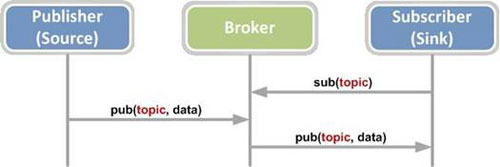
\includegraphics[scale=0.8]{publish_subscribe.jpg}
\end{figure}

Il protocollo si presta particolarmente all'Internet of Things per via di una serie di vincoli ai quali questa nuova realtà è sottoposta come connessione di dispositivi meno sofisticati rispetto a quelli connessi ad internet, spesso embedded, con richiesta di \textbf{impiego minimo di risorse energetiche}, \textbf{minore flessibilità computazionale} e quindi capacità più limitate, oltre che\textbf{ maggiore accessibilità economica}. MQTT dunque si adatta a tali necessità grazie alle sue principali caratteristiche: \textbf{leggero}, \textbf{semplice da implementare} ed \textbf{efficiente} in ambienti in cui la rete consente una larghezza di banda limitata.

Per ciò che concerne l'aspetto tecnico, MQTT viaggia su \textbf{protocollo di rete TCP/IP} e ha \textbf{bassi overhead di trasporto}, grazie anche ad un formato di messaggio con header fissato a 2 bytes, che è anche la dimensione minima di un pacchetto. MQTT fornisce tre tipi di \textbf{Quality of Service}. 
\\I tre livelli di servizio sono:
\begin{itemize}
	\item  \textbf{At most once} (al più una volta): i messaggi vengono consegnati in base al miglior effort di rete, per cui possono avvenire perdite o repliche di informazione;
	\item \textbf{At least once} (almeno una volta): si assicura l’arrivo del messaggio, ma possono avvenire repliche;
	\item \textbf{Exactly once} (esattamente una volta): si assicura che i messaggi arrivino esattamente una volta.
\end{itemize}

\subsection{Obiettivi}

Il protocollo descritto è stato utilizzato per implementare un Arduino come client MQTT che invia ad un broker, su di un certo topic, i dati rilevati dal sensore giroscopio-accelerometro, il quale poi rendirizza tali informazioni a tutti i client connessi al broker che sottoscrivono il topic.

\section{Tecnologie}
\subsection{Materiale}
Il materiale utilizzato per lo sviluppo del progetto è il seguente: 
\begin{itemize}
	\item Arduino Uno
	\item Ethernet Shield
	\item Sensore MPU-6050 (Giroscopio – Accelerometro) 
\end{itemize}	
\subsection{Librerie e Tool}
Per quel che concerne il materiale software, l'attenzione si è focalizzata fondamentalmente su alcune librerie per Arduino e sul server usato come broker.

\subsubsection{Librerie} 
\begin{itemize}
	\item \textbf{Wire.h}: libreria contenente funzioni che agevolano l’utilizzo del \textbf{protocollo I2C} (sistema di comunicazione seriale, che prevede un "Master"  ed uno o più "Slave"). Ovviamente, nella nostra configurazione, Arduino assume il ruolo di master ed il \emph{MPU-6050} funge da slave, ricevendo le richieste e fornendo le relative risposte
	\item \textbf{SPI.h}
	\item \textbf{Ethernet.h}: libreria che permette l'accesso a internet di Arduino tramite ethernet.
	\item \textbf{PubSubClient.h}: questa libreria fornisce un serie di funzioni per creare un client MQTT
\end{itemize}

\subsubsection{Il broker utilizzato: Mosquitto}
Mosquito (\textbf{http://mosquitto.org/}) è un Message Broker open source (EPL / EDL licenza) che implementa la versione del protocollo MQTT 3.1 e 3.1.1.

Mosquitto è realizzato in C ed è un server molto leggero. E' stato sviluppato dallo stesso gruppo che ha fornito il codice client ad Eclipse.org per dar vita al progetto Paho.

La sua semplicità di realizzazione gli permette di essere supportato praticamente da qualsiasi sistema Linux, Windows, Mac. Essere scritto in C gli permette di essere utilizzato praticamente ovunque.
\newpage
\section{Implementazione}
Il primo step è stato configurare Arduino come nello schema seguente (Figure 1).
\begin{figure}[h]
	\centering
	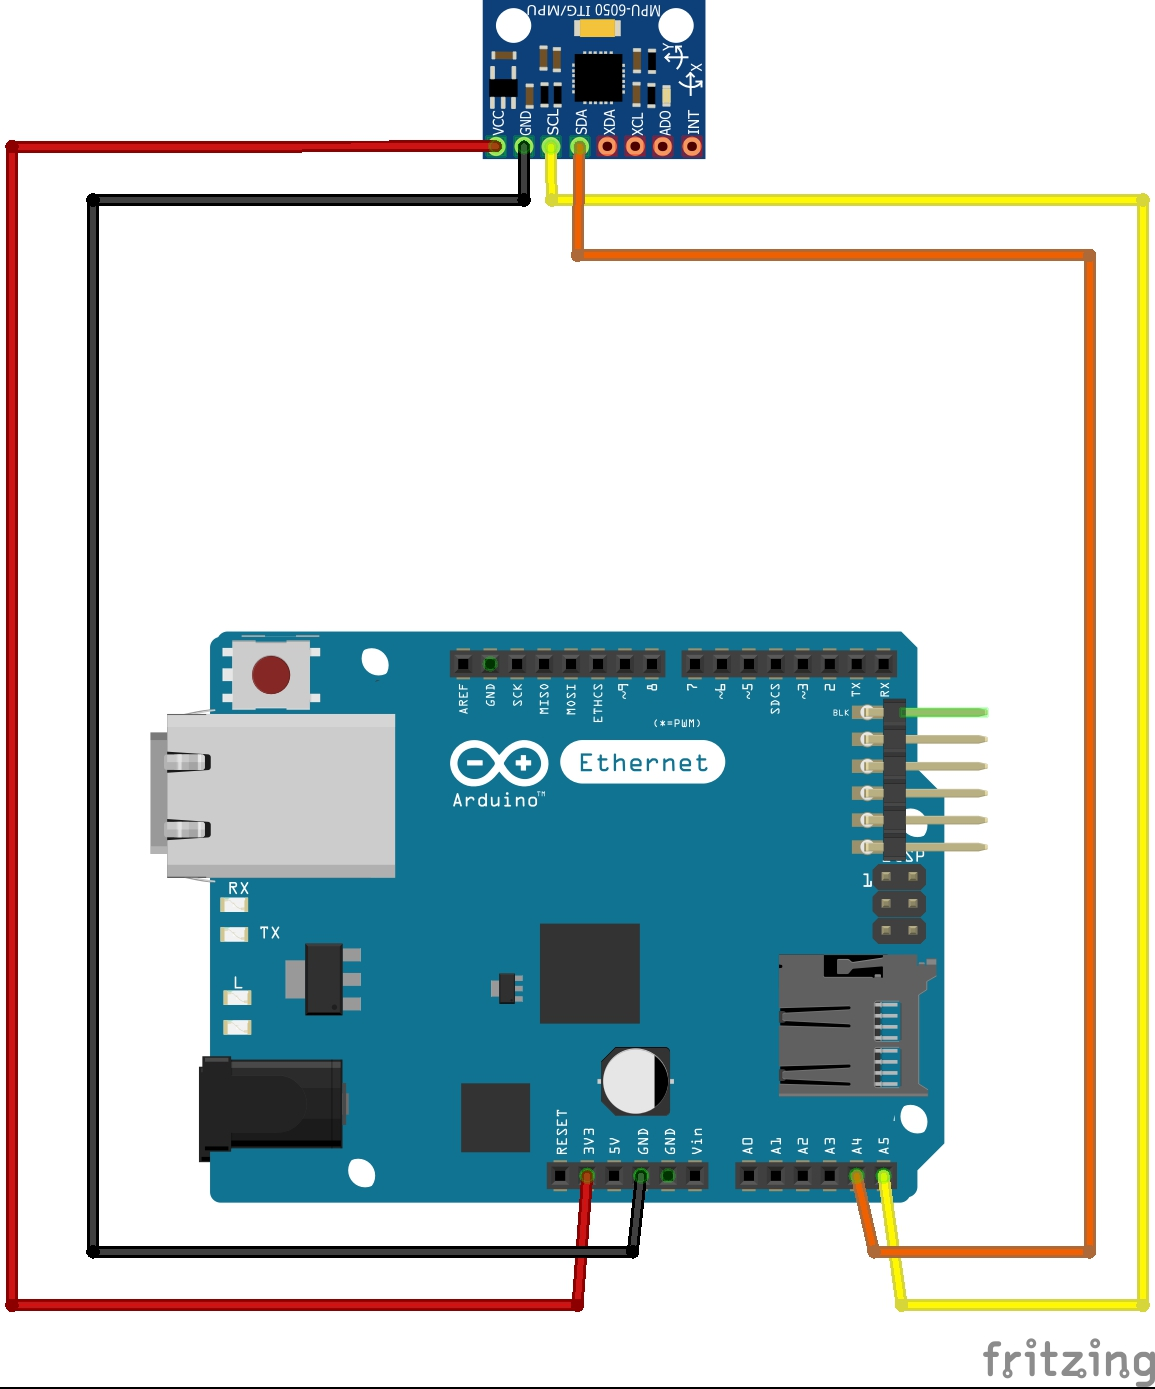
\includegraphics[scale=0.7]{fritzing_bb.jpg}
	\caption{Schema Arduino}
\end{figure}
\\
Arduino è stato programmato come client MQTT che dapprima rileva i valori del sensore Giroscopio/Accelerometro. Successivamente si connette al server Mosquitto, in esecuzione su di un'altra macchina alla quale i valori vengono inviati creando due topic: uno per i valori dell'accelerometro e uno per i valori del giroscopio.
Arduino funge quindi da client publisher, inviando al server i valori in tempo reale attraverso due topic distinti.
\\
Mosquitto quindi si occupa di inviare i messaggi a tutti i subscriber dei due topic.
Al momento, i client testati, sono dei client MQTT tool che consentono di connettersi a un broker, oppure dei client mosquitto creati da linea di comando attraverso un shell.

\subsection{Code}

\subsubsection{Arduino}

Di seguito sono mostrati i punti salienti del codice dello sketch Arduino.\\\\
All'interno del setup viene eseguito il seguente codice, nel quale inizializziamo la trasmissione dei dati tra il sensore ed Arduino, settiamo il server al quale Arduino invierà i valori e assegnamo un indirizzo IP allo shield ethernet: \\

\begingroup
\fontsize{9.5pt}{8pt}\selectfont
\begin{lstlisting}[frame=single]
EthernetClient ethClient;
PubSubClient mqttClient(ethClient);

void setup(){

  Wire.begin();
  Wire.beginTransmission(MPU);
  Wire.write(0x6B);  // PWR_MGMT_1 register
  Wire.write(0);     // set to zero (wakes up the MPU-6050)
  Wire.endTransmission(true);

  mqttClient.setServer(server, 1883);

  Ethernet.begin(mac);
  ip = Ethernet.localIP();

  delay(1500);
}
\end{lstlisting}
\endgroup

Il loop che viene eseguito è invece il seguente; viene invocata la funzione dataReceiver(), che si occupa della lettura dei dati, quindi Arduino tenta di collegarsi come client MQTT al server con le configurazioni precedentemente descritte e nel caso non vada a buon fine, tenta di riconnettersi. Una volta connesso, l'MQTT client loop viene invocato per far sì che venga mantenuta la connessione e periodicamente si controlli la presenza di nuovi messaggi in entrata. Quindi vengono richiamate le funzioni dataAccProducer() e dataGYProducer() che invece si occupano di inviare i messaggi al server contenenti i dati letti dal sensore (dataAccProducer() per quelli relativi all'accelerometro e dataGYProducer() per quelli del giroscopio).

\begingroup
\fontsize{9.5pt}{8pt}\selectfont
\begin{lstlisting}[frame=single]
void loop(){

  dataReceiver();
  if (!mqttClient.connected()) {
    reconnect();
  }
  mqttClient.loop(); 
  dataAccProducer();
  dataGyProducer();

  delay(50);
}
\end{lstlisting}
\endgroup
\newpage
La funzione mostrata di seguito è quella che consente la lettura dei dati dal sensore.
\begingroup
\fontsize{9.5pt}{8pt}\selectfont
\begin{lstlisting}[frame=single]
void dataReceiver(){
   Wire.beginTransmission(MPU);
   Wire.write(0x3B);  (ACCEL_XOUT_H)
   Wire.endTransmission(false);
   Wire.requestFrom(MPU,14,true); 
   AcX = Wire.read()<<8|Wire.read(); 
   AcY = Wire.read()<<8|Wire.read();  
   AcZ = Wire.read()<<8|Wire.read(); 
   GyX = Wire.read()<<8|Wire.read();  
   GyY = Wire.read()<<8|Wire.read(); 
   GyZ = Wire.read()<<8|Wire.read(); 
   processData();
}
\end{lstlisting}
\endgroup

Le seguenti sono invece le funzioni che producono i messaggi; nella prima parte della funzione viene creato un array di caratteri contenente i valori letti dal sensore accelerometro. L'array di caratteri viene quindi utilizzato come parametro della funzione MQTTClient.publish("Acc", concatenazione) che invia il messaggio al broker:

\begingroup
\fontsize{9.5pt}{8pt}\selectfont
\begin{lstlisting}[frame=single]
void dataAccProducer(){

  char concatenazione[100]= "X = ";   
  strcat(concatenazione,init(gForceX));
  strcat(concatenazione," | Y = ");
  strcat(concatenazione,init(gForceY));
  strcat(concatenazione," | Z = ");
  strcat(concatenazione,init(gForceZ));

  mqttClient.publish("Acc", concatenazione);
}
\end{lstlisting}
\endgroup

Speculare è la funzione per i dati del giroscopio:

\begingroup
\fontsize{9.5pt}{8pt}\selectfont
\begin{lstlisting}[frame=single]
void dataGyProducer(){

  char concatenazione[100]= "X = ";
  strcat(concatenazione,init(rotX));
  strcat(concatenazione," | Y = ");
  strcat(concatenazione,init(rotY));
  strcat(concatenazione," | Z = ");
  strcat(concatenazione,init(rotZ));
  
  mqttClient.publish("Gy",concatenazione);
}
\end{lstlisting}
\endgroup

\subsubsection{Client Java}

Come descritto nei paragrafi precedenti, i dati rilevati dal sensore giroscopio-accelerometro, vengono inviati al broker MQTT Mosquitto il quale si occupa di reindirizzarli a tutti i client a lui connessi che sottoscrivono i topic sui quali questi sono stati pubblicati. Abbiamo quindi implementato un client Java che si occupa di ricevere i messaggi, gestire i dati ricevuti, e rappresentarli all'interno di alcuni grafici.

Di seguito sarà mostrato l'implementazione di quanto brevemente descritto .
Innanzitutto, per la creazione del client MQTT è stata utilizzata la libreria \textbf{Eclipse Paho}, che consente la comunicazione M2M tramite protocollo MQTT.
Di seguito viene mostrata la parte di codice che crea la connessione al server Broker:

\begingroup
\fontsize{9.5pt}{8pt}\selectfont
\begin{lstlisting}[frame=single]
public void connectAndSubscribe() {
  try {
    client = new mqttClient("tcp://indirizzoServer:porta", "NomeClient");
    client.connect();
    client.setCallback(this);
    client.subscribe("Acc");
    client.subscribe("Gy");
  } 
  catch (mqttException e) {
    e.printStackTrace();
  }
}
\end{lstlisting}
\endgroup

Come possiamo vedere nelle prime righe del codice viene eseguita la connessione al server indicato, viene quindi effettuata la sottoscrizione per i due topic che riguardano i dati dell'accelerometro e del giroscopio.

Tutto ciò viene realizzato attraverso un'interfaccia grafica che, una volta connessa al server, inizia a disegnare i grafici riguardanti gli assi \textbf{x},\textbf{y},\textbf{z} dell'accelerometro e del giroscopio in relazione con il \textbf{tempo} (figura 2).

\begin{figure}[h]
	\centering
	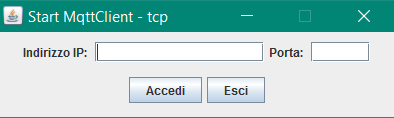
\includegraphics[scale=0.8]{login.jpg}
	\caption{Login Client}
\end{figure}
 \newpage
\begin{figure}[h]
	\centering
	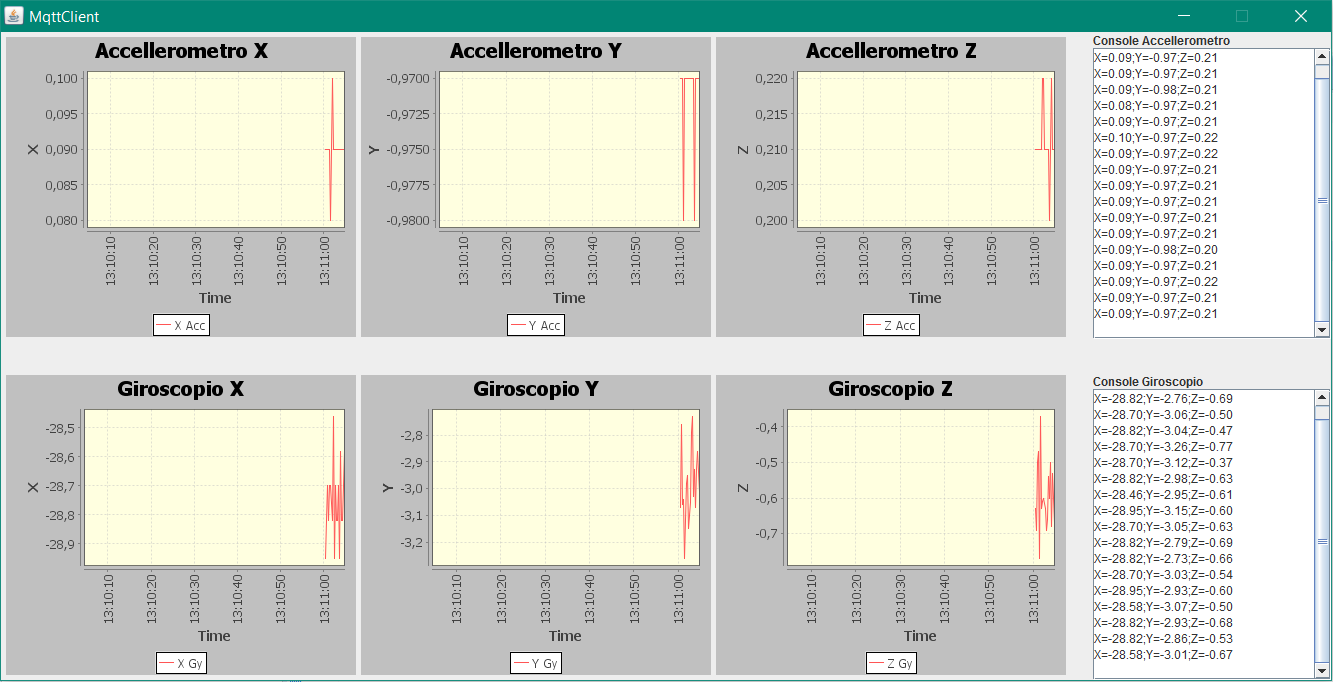
\includegraphics[scale=0.3]{gui.png}
	\caption{Interfaccia Client Java}
\end{figure}

Dapprima viene richiesto l'inserimento dell'indirizzo IP e la porta del server, successivamente vengono mostrati i grafici relativi ai nostri sensori e due console nelle quali vengono illustrati i dati così come vengono sottoscritti sul broker.

\begin{figure}[ht]
	\centering
	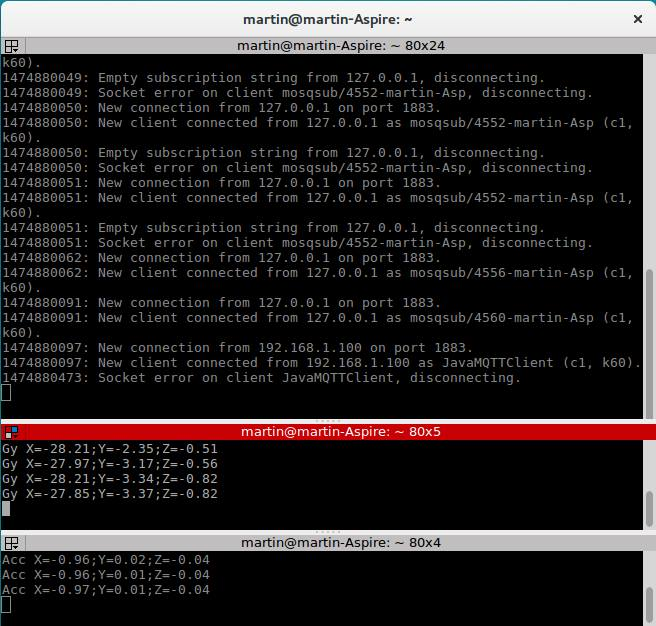
\includegraphics[scale=0.3]{broker.png}
	\caption{Sottoscrizione dei dati sul broker Mosquitto}
\end{figure}
All'arrivo di ogni messaggio, il client si occupa di elaborare i dati contenuti al suo interno in modo da ottenere dei valori utilizzabili per la rappresentazione dei grafici. 
\newpage
\begingroup
\fontsize{9.5pt}{8pt}\selectfont
\begin{lstlisting}[frame=single]
@Override
public void messageArrived(String topic, mqttMessage message) {
  double x = 0;
  double y = 0;
  double z = 0;

  String[] parts = message.toString().split(";");

  for(int i=0; i<parts.length; i++){
    String[] temp=parts[i].split("=");

  	switch (temp[0]) {
        case "X":
          x = Double.parseDouble(temp[1]);
          break;
        case "Y":
          y = Double.parseDouble(temp[1]);
          break;
        case "Z":
          z = Double.parseDouble(temp[1]);
          break;
        default:
          break;
    }			
  }

  if(topic.equals("Acc")){						
     xAcc = x;
     yAcc = y;
     zAcc = z;
     msgAcc = new String(message.toString()+"\n");
  }
  else if(topic.equals("Gy")){
     xGy = x;
     yGy = y;
     zGy = z;
     msgGy = new String(message.toString() + "\n");		
  }
}
\end{lstlisting}
\endgroup
Per quanto riguarda l'interfaccia grafica, è stata realizzata mediante l'utilizzo delle librerie \textbf{AWT} e \textbf{SWING}, mentre grazie a \textbf{JFREE CHART} sono stati disegnati i grafici.

\newpage
\section{Installazione}
 
Come descritto nelle sezioni precedenti affinchè tutto funzioni correttamente è necessario che tutto venga correttamente installato e configurato.

Innanzitutto è necessario connettere sulla stessa rete tramite cavo ethernet (se non dotato di connessione wireless) la macchina sulla quale viene lanciato il server, la macchina sulla quale viene avviato il client ed Arduino Uno.

Collegato correttamente quanto elencato è necessario installare il broker Mosquitto su di una macchina (preferibilmente Linux per semplicità d'uso).
L'installazione di Mosquitto su di una macchina Windows, può essere effettuata seguendo pedissecuamente passo dopo passo la guida raggiungibile attraverso il link di seguito indicato:
\\
"https://sivatechworld.wordpress.com/2015/06/11/step-by-step-installing-and-config\\uring-mosquitto-with-windows-7/"
\\

Altrimenti è consigliato installare per semplicità il server su di una macchina Linux con i seguenti comandi:

\begingroup
\fontsize{9.5pt}{8pt}\selectfont
\begin{lstlisting}[frame=single]
$apt-get update
$apt-get install build-essential libwrap0-dev libssl-dev libc-ares-dev uuid-dev xsltproc
\end{lstlisting}
\endgroup

Una volta installato sarà possibile quindi lanciare il server semplicemente attraverso il comando "mosquitto".

A questo punto è quindi necessario configurare Arduino Uno, settando all'interno del file .ino l'indirizzo ip sul quale è stato lanciato il server, modificando i valori all'interno della seguente riga di codice:

\begingroup
\fontsize{9.5pt}{8pt}\selectfont
\begin{verbatim}
  IPAddress server(xxx, xxx, xxx, xxx);
\end{verbatim}
\endgroup

Una volta caricato il codice all'interno della memoria di Arduino, è sufficiente lanciare su di un'altra macchina il file .jar contenente il client MQTT, inserire nell'interfaccia grafica l'indirizzo ip del server e la porta ed avviarlo, instaurando quindi una connessione con il server e ponendosi in attesa di messaggi in arrivo.
\newpage
\begin{thebibliography}{argomento}

\bibitem[Arduino]{etichetta} \emph{Arduino - Introduction}, \url{http://arduino.cc/en/guide/introduction}
\bibitem[Arduino Uno]{etichetta} \url{https://www.arduino.cc/en/Main/ArduinoBoardUno}
\bibitem[Arduino, MPU-6050]{etichetta} \url{http://www.giuseppecaccavale.it/arduino/mpu-6050-gy-521-arduino-tutorial/}
\bibitem[MQTT Protocol]{etichetta} \url{http://mqtt.org/}
\bibitem[Mosquitto]{etichetta} \url{https://mosquitto.org/}
\bibitem[SPI library, Arduino]{etichetta} \url{https://www.arduino.cc/en/Reference/SPI}
\bibitem[Ethernet library, Arduino]{etichetta} \url{https://www.arduino.cc/en/Reference/Ethernet}
\bibitem[Wire library, Arduino]{etichetta} \url{https://www.arduino.cc/en/Reference/Wire}
\bibitem[PubSubClient library, Java]{etichetta} \url{http://pubsubclient.knolleary.net/}
\bibitem[Eclipse Paho library, Java]{etichetta} \url{https://eclipse.org/paho/}
\bibitem[JFreeChart library, Java]{etichetta} \url{http://www.jfree.org/jfreechart/}
\bibitem[Swing library, Java]{etichetta} \url{https://docs.oracle.com/javase/7/docs/api/javax/swing/package-summary.html}
\end{thebibliography}
\end{document}